
\subsection{I-doit}

Bei I-doit handelt es sich um eine von \textit{synetics} entwickelte webbasierte Software, die zur Abbildung komplexer IT-Infrastrukturen dient.
Dabei stehen dem Anwender verschiedene Komponenten zur Verfügung. 
Die aktuelle Version ist dabei 1.4.8 (31.Oktober 2014). 

Die zentrale Komponente, die sogenannte \textit{Configuration Management Database (CMDB)} dient dabei dem Nutzer zum anlegen verschiedener Objekte, wie z.B. Workflows, IT-Systeme, Kontakte und Services.
Weitere Komponenten wie Import oder Export sind ebenfalls enthalten.
Ein Reportmanager erleichtert den Umgang mit dokumentierten Daten. 
Durch die Plattformunabhängigkeit und die standardisierten Programmiersprachen PHP, MySQL und Javascript wird ein flexibler Einsatz gewährleistet.

I-doit ist in zwei Versionen verfügbar. Zum Einen eine frei verfügbare Open-Source Version und zum Anderen eine kostenpflichtige Pro Version.
Die Unterschiede sowie die verschiedenen Preise in Hinblick auf die Pro Version sind in Abbildung~\ref{fig:idoitvergleich} und Abbildung~\ref{fig:idoitpreis} einsehbar.

\begin{figure}[htbp]
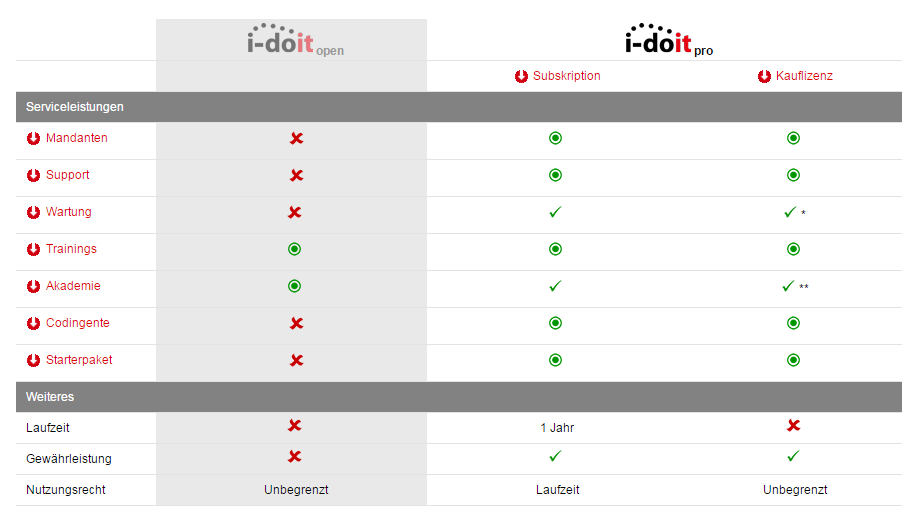
\includegraphics[width=\textwidth]{images/idoitvergleich}
\caption{Vergleich der Versionen von I-doit im Vergleich}
\label{fig:idoitvergleich}
\end{figure}

\begin{figure}[htbp]
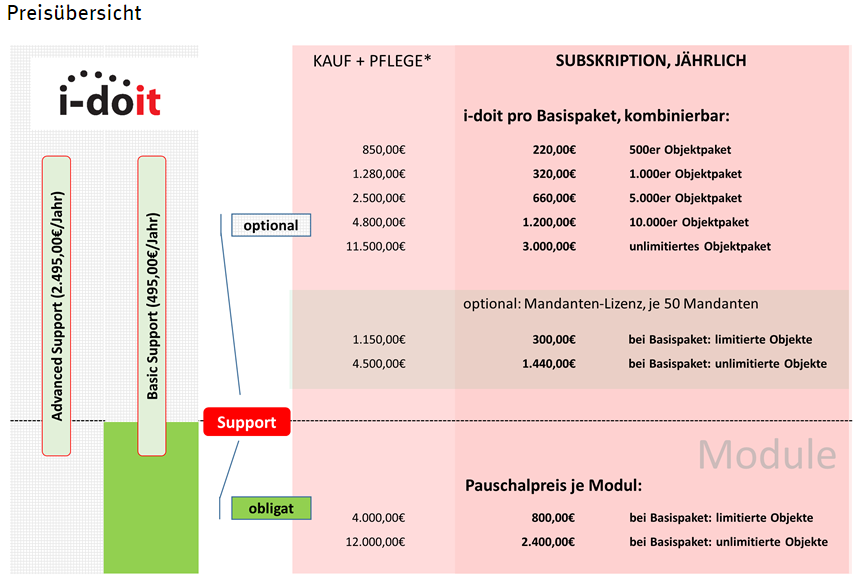
\includegraphics[width=\textwidth]{images/idoitpreis}
\caption{Preise der Versionen von I-doit im Vergleich}
\label{fig:idoitpreis}
\end{figure}

Durch ein Rechtesystem sind administrative Regelungen problemlos möglich, da verschiedene Rollen vergeben werden können.
Das bedeutet, Anwender können einer Personengruppe zugeordnet werden, die verschiedene Rechte wie Lese-, Schreib- oder Administrationsrechte beinhalten.

Ein weiteres Feature von I-doit ist die Mandantenfähigkeit, wodurch innerhalb einer I-doit Instanz verschiedene Mandanten komplett voneinander getrennt entworfen werden können.
Bei der Erzeugung von Objekten wird der Anwender durch Templates unterstützt.
So können z.B. verschiedene Rechner vom gleichen Typ mehrfach abgebildet werden, ohne alle einzeln zu erstellen.

Das Reporting von I-doit, welches auf den I-doit Datenbanken basiert, ermöglicht ein automatisiertes Erstellen und Auswerten der eingetragenen Objekte.
In den Reports werden wichtige Eckdaten wie Statistiken zur abgebildeten Infrastruktur zusammengefasst.
Dabei stehen die Formate Text, PDF, CSV und XML zur Verfügung.

Ein wesentlicher Unterschied, den wir ohne eine Testversion der kostenpflichtigen Variante von I-doit feststellen konnten, liegt in der Sprachunterstützung.
Die Open-Source Version ist lediglich in englischer Sprache verfügbar, wohingegen die Pro Version mehrsprachig entwickelt wurde.


\subsubsection{Umsetzung des Fallbeispiels}
Nachfolgend sind in Abbildung~\ref{fig:idoittree} und Abbildung~\ref{fig:idoitschema} die Resultate der Übertragung des Fallbeispiels nach I-doit zu sehen.
Darauf zu sehen ist die Infrastruktur, die durch das Fallbeispiel definiert ist, mit den entsprechenden Objekten und deren Verknüpfungen.
Abbildung~\ref{fig:idoittree} zeigt die Standortansicht, in der die Objekte hinzugefügt und angelegt werden, wohingegen Abbildung~\ref{fig:idoitschema} die CMDB Ansicht darstellt.
Aus Platzgründen konnte die schematische Darstellung von Abbildung~\ref{fig:idoitschema} hier nicht vollständig dargestellt werden.

\begin{figure}[htbp]
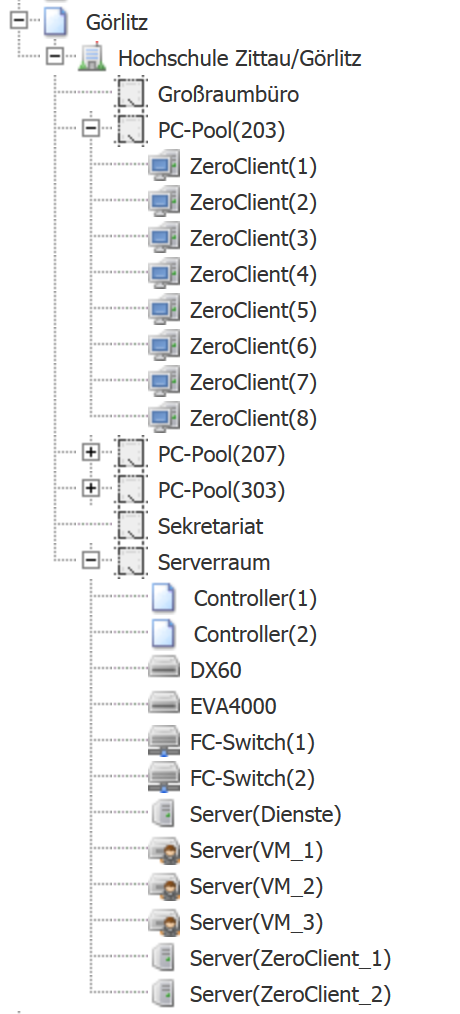
\includegraphics[scale=1]{images/idoittree}
\caption{Baumstruktur in I-doit}
\label{fig:idoittree}
\end{figure}

\begin{figure}[htbp]
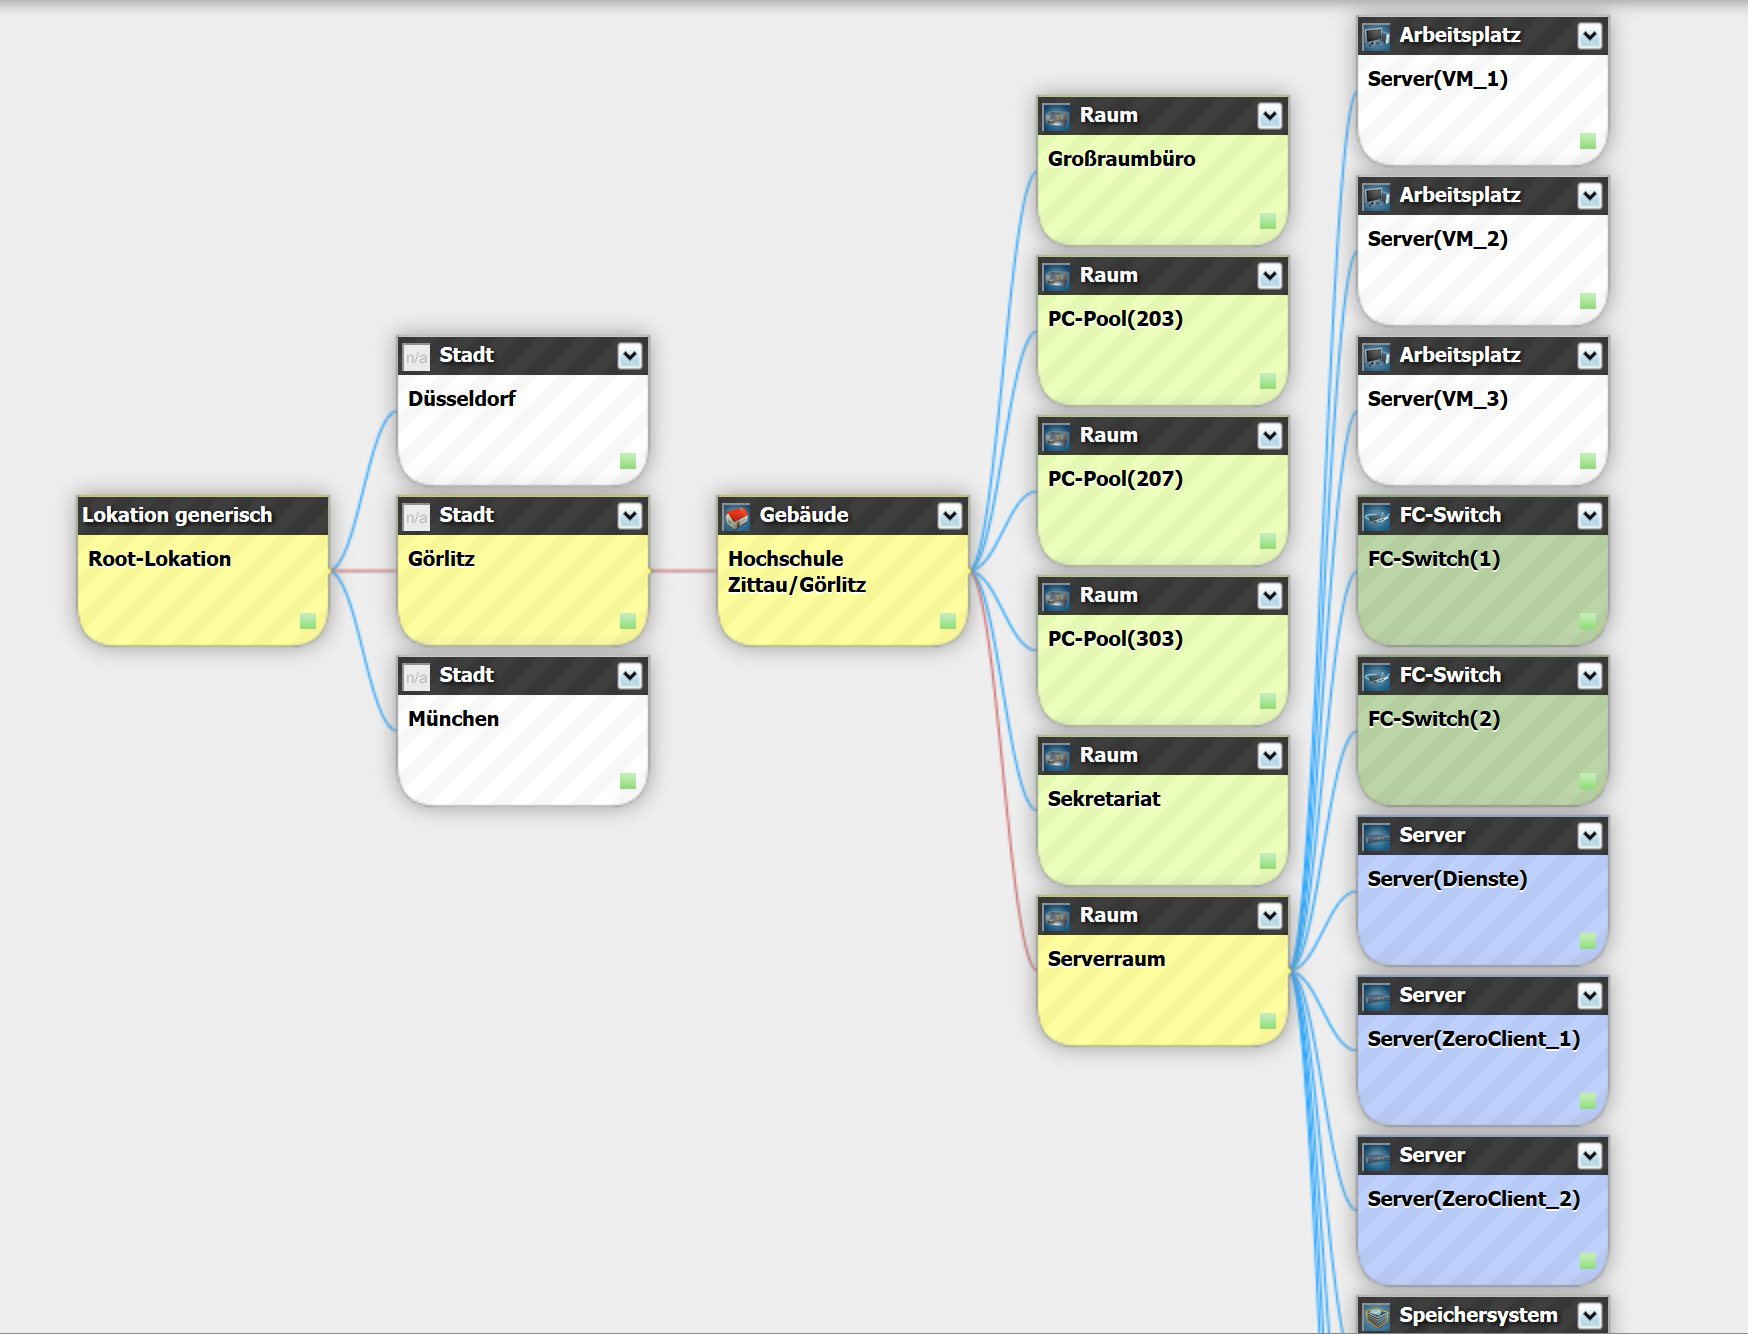
\includegraphics[width=\textwidth]{images/idoitschema}
\caption{Infrastrukturdarstellung in I-doit}
\label{fig:idoitschema}
\end{figure}


\subsubsection{Bewertungsergebnisse}
Tabelle~\ref{tab:BerwertungIdoit} zeigt die Punkteverteilung für das Tool I-doit. 
Die möglichen Bereiche spannen sich von 0 (nicht vorhanden) bis 10 (sehr gut).
Allgemein betrachtet erzielte I-doit eine gute Gesamtbewertung mit 221 von maximal 280 erreichbaren Punkten.
Gemäß der vorher festgelegten Wichtungen eignet sich I-doit damit mit ca. $82,5\%$ für den Gebrauch durch die Hochschule und mit ca. $83,4\%$ für den Gebrauch für die Lehre
an der Hochschule.

Negativ kristallisierten sich Aspekte im Bereich der Vererbung heraus. Hier wurden Werte bezüglich der Integrität, der Authentizität und der Verfügbarkeit nicht an Elternelemente vererbt. Andere Werte, wie der Zustand der Objekte, wurden dagegen weitergegeben.
Ein weiterer negativer Aspekt ist die Funktion zum Export von Berichten. Hierbei ist die Flexibilität für die Erstellung eines Reports nur sehr beschränkt möglich.
Auch die Risikobewertung, welche die aktuelle Situation der Infrastruktur bewerten soll, war nur begrenzt vorhanden. 

Die Usabilty von I-doit wird unterstützt durch zahlreiche Templates. Nichtsdestotrotz ist die Menüführung für die Erstellung und Verknüpfung von Objekten nicht intuitiv und bringt eine längere Einarbeitungszeit mit sich.

\begin{table}[h]
%\centering
\begin{tabular}{|p{0.5\textwidth}|p{0.5\textwidth}|}
\hline
Kriterium & Bewertung\\
\hline
\textbf{GUI}& \\
\hline
Wizard & 5 \\
\hline
Infrastrukturdarstellung & 10 \\
\hline
Netzpläne & 6 \\
\hline
Prozessflüsse & 8 \\
\hline
Schnelles Einpflegen von Änderungen & 7 \\
\hline
\textbf{Objektrelationen} &  \\
\hline
Doppelseitige Verlinkungen & 10 \\
\hline
Vererbung & 4 \\
\hline
Gruppierungen & 10 \\
\hline
\textbf{Funktionalität} &\\
\hline
Aktuelle BSI-Standards & 10 \\
\hline
Erweiterbarkeit der Klassifizierungen & 10 \\
\hline
Individuelle Beschreibungen & 10 \\
\hline
Sicherheitsverstöße markieren & 8 \\
\hline
Bewertung des Sicherheitsstatus & 10 \\
\hline
Export von Berichten & 5 \\
\hline
BSI-Toolimport & 10 \\
\hline
Sicherheit des Tools an sich & 8 \\
\hline
Risikobewertung & 5 \\
\hline
\textbf{System}& \\
\hline
Verteiltes Arbeiten & 10 \\
\hline
Rechtevergabe & 10 \\
\hline
Kosten & 10 \\
\hline
Support & 10 \\
\hline
Zertifizierung & 10 \\
\hline
Dokumentation & 5 \\
\hline
Marktpräsenz & 10 \\
\hline
Spezielle Zielgruppe & 10 \\
\hline
Pflege/Weiterentwicklung & 10 \\
\hline
\multicolumn{2}{c}{}\\
\hline
\textbf{Gesamt} & 221\\
\hline
Hochschuleinsatz & $82,5\%$\\
\hline
Lehre & $83,4\%$\\
\hline
\end{tabular}
\caption{Bewertung: I-doit}
\label{tab:BerwertungIdoit}
\end{table}



\subsection{Audit-Tool 2009}
Beim \textit{Audit-Tool~2009} handelt es sich um ein Produkt der Firma \textit{Secure-IT}.
Auf der Website wird damit geworben, dass sich das Tool für eine grobe Strukturanalyse und eine grobe Modellierung eignet.
Weiterhin wird damit geworben, dass das Tool das aktuelle Sicherheitsniveau anzeigt. Auch sollen die Stärken und Schwächen  der
eigenen IT-Sicherheit angezeigt werden.
Im Abschluss verspricht die Website ebenfalls die Ermittlung der Komponenten für die der 
größte Handlungsbedarf besteht.

Das Tool konnte nicht ausprobiert und bewertet werden, da die Firma keine Testversion bereitgestellt hat.
Es wurden wiederholt Mails an die Firma geschrieben, auf die nicht geantwortet wurde.
Auch der telefonische Kontakt konnte nicht hergestellt werden, da auch bei mehrfachen Versuchen niemand abgenommen hat.
Die letzte Aktualisierung auf der Website fand ende 2012 statt.


\subsection{Verinice}
Verinice ist eine freie und Open-Source-Informationssicherheitsmanagementsystem (ISMS) Anwendung, die bei der Schaffung und Erhaltung von Systemen des Informations- und Sicherheitsmanagements helfen kann.

Verinice wurde von einer deutschen Firma SerNet Service Network GmbH geschrieben und wird gleichzeitig gepflegt.

Verinice steht unter der GNU General Public License (Version 3 oder höher).

Zu den wichtigsten Nutzern gehören kleine und mittlere Unternehmen, einige große Unternehmen und Regierungsbehörden.

In Deutschland wird Verinice als ISMS Tool vom Verband der Automobilindustrie empfohlen
für ihre Mitglieder wie Volkswagen, Daimler AG, Fiat und andere großen Herstellern.
VDA fördert auch Verinice Entwicklung seit Release 1.2.

Verinice unterstützt die Betriebssysteme Windows, Linux und OS X.

\begin{figure}[htbp]
	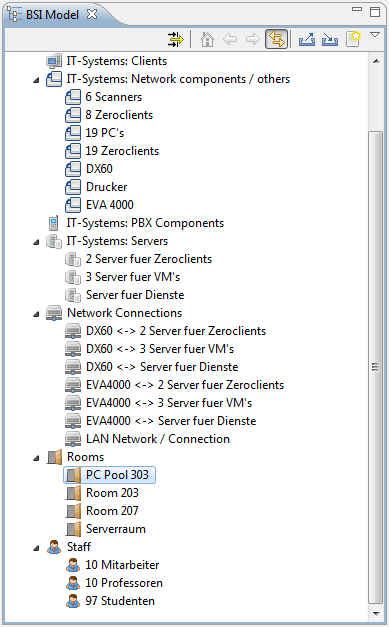
\includegraphics[scale=0.5]{images/verinicestruktur}
	\caption{Infrastrukturdarstellung in Verinice}
	\label{fig:veriniceStruktur}
\end{figure}


\begin{table}[h]
%\centering
\begin{tabular}{|p{0.5\textwidth}|p{0.5\textwidth}|}
\hline 
Kriterium & Bewertung\\ 
\hline 
\textbf{GUI}& \\
\hline
Wizard & 5\\
\hline 
Infrastrukturdarstellung & 7 \\
\hline 
Netzpläne & 0 \\
\hline 
Prozessflüsse & 0 \\
\hline 
Schnelles Einpflegen von Änderungen & 10 \\
\hline
\textbf{Objektrelationen} & \\
\hline 
Doppelseitige Verlinkungen & 10 \\
\hline 
Vererbung & 0 \\
\hline 
Gruppierungen & 10 \\
\hline 
\textbf{Funktionalität} &\\
\hline 
Aktuelle BSI-Standards & 10 \\
\hline  
Erweiterbarkeit der Klassifizierungen & 10 \\
\hline 
Individuelle Beschreibungen & 10 \\
\hline 
Sicherheitsverstöße markieren & 5 \\
\hline
Bewertung des Sicherheitsstatus & 5 \\
\hline
Export von Berichten & 10 \\
\hline
BSI-Toolimport & 10 \\
\hline
Sicherheit des Tools an sich & 8 \\
\hline
Risikobewertung & 5 \\
\hline
\textbf{System}&  \\
\hline
Verteiltes Arbeiten & 10 \\
\hline
Rechtevergabe & 10 \\
\hline
Kosten & 9 \\
\hline
Support & 10 \\
\hline
Zertifizierung & 10 \\
\hline
Dokumentation & 5 \\
\hline
Marktpräsenz & 10 \\
\hline
Spezielle Zielgruppe & 5 \\
\hline
Pflege/Weiterentwicklung & 6 \\
\hline
\multicolumn{2}{c}{}\\
\hline
\textbf{Gesamt} & 190\\
\hline
Hochschuleinsatz & $71,8\%$\\
\hline
Lehre & $64,0\%$\\
\hline
\end{tabular} 
\caption{Bewertung: Verinice}
\label{tab:BerwertungVerinice}
\end{table}







